\documentclass[a4paper,11pt]{article}

\usepackage{setspace}
\onehalfspacing

\usepackage[utf8]{inputenc}
\usepackage[T1]{fontenc}
\usepackage[english]{babel}

\usepackage{color}
\usepackage{float}
\usepackage{fancyvrb}

\usepackage{amssymb}
\usepackage{amsmath}
\usepackage{listings}
\usepackage{comment} 

\usepackage{caption}
\usepackage{subcaption}

\usepackage{graphicx}
\DeclareGraphicsExtensions{.jpg}

\definecolor{dkgreen}{rgb}{0,0.45,0}
\definecolor{gray}{rgb}{0.5,0.5,0.5}
\definecolor{mauve}{rgb}{0.30,0,0.30}

\lstset{frame=tb,
  language=Python,
  aboveskip=3mm,
  belowskip=3mm,
  showstringspaces=false,
  columns=flexible,
  basicstyle={\small\ttfamily},
  numbers=left,
  numberstyle=\footnotesize,
  keywordstyle=\color{dkgreen}\bfseries,
  commentstyle=\color{dkgreen},
  stringstyle=\color{mauve},
  frame=single,
  breaklines=true,
  breakatwhitespace=false,
  tabsize=4
}

\begin{comment}
\begin{lstlisting}[language=python]
her kan i vise kode som i forklarer.
indryk virker fint her.
\end{lstlisting}
\end{comment}

\title{First year project\\Project 99: Who's Julia?\\\rule{10cm}{0.5mm}}
\author{Group: 99a\\Simon Lehmann Knudsen, simkn15\\Sonni Hedelund Jensen, sonje15\\Asbjørn Mansa Jensen, asjen15
	\\ DM501\\\rule{5.5cm}{0.5mm}\\}
\date{\today}

\begin{document}

\maketitle

\vfill

\newpage
\tableofcontents

\newpage
\section{Introduction}
Julia is a new open source object orientated programming language which shares many similarities with python. The language is made for high performance and scientific computations while still supporting general purpose programming. 
Programming in Julia can be done in the terminal like python with interactive mode:
\begin{figure}[H]
	\centering
	\begin{subfigure}[b]{0.8\textwidth}
		\centering
		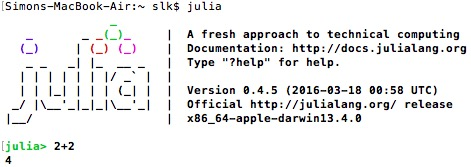
\includegraphics
		[width=\textwidth]{terminalj.jpg} 
		\caption{Julia}.
	\end{subfigure}	
	\begin{subfigure}[b]{0.8\textwidth}
		\centering
		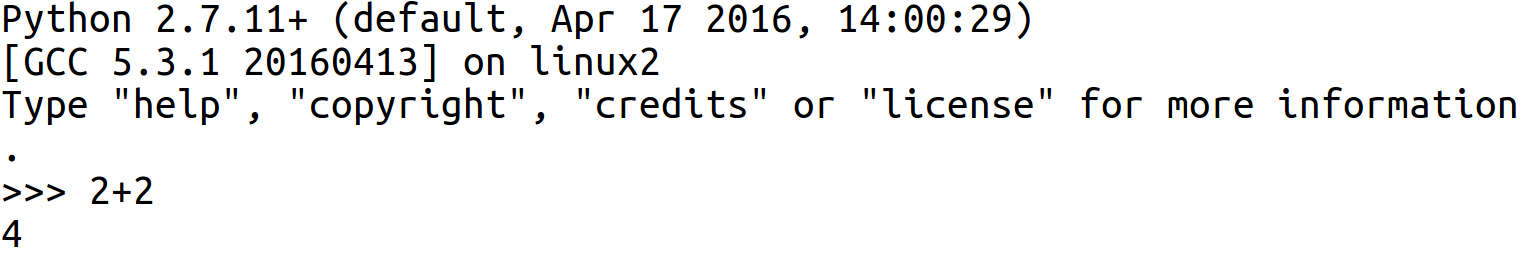
\includegraphics
		[width=\textwidth]{terminalp.jpg} 
		\caption{Python}.
	\end{subfigure}
	\caption{Julia in terminal}
\end{figure}
Writing longer programs in the terminal might not be the preferred method. The text editor Atom supports the Julia language. Atom has a package, \textbf{uber-juno}, which sets up Atom to act like an IDE, integrated development environment for Julia.

\subsection{Syntax}
\textit{Make examples of syntax between all the languages here}.

\begin{figure}[H]
	\begin{lstlisting}[language=python]
	Julia:	    Python:      Java:            c++:
	a = 10	    a = 10       int a = 10;      int a = 10;
	\end{lstlisting}
	\caption{Declaring variables}
	\label{variables}
\end{figure}

\begin{figure}[H]
	\centering
	\begin{subfigure}[b]{0.7\textwidth}
		\centering
		\begin{lstlisting}
		for i = 1 : 10
			println(i)
		end
		\end{lstlisting}
		\caption{Julia}
	\end{subfigure}
	\begin{subfigure}[b]{0.7\textwidth}
		\centering
		\begin{lstlisting}
		for i in range(1, 11)
			print i
		\end{lstlisting}
		\caption{Python}
	\end{subfigure}	
	\begin{subfigure}[b]{0.7\textwidth}
		\centering
		\begin{lstlisting}
		for (int i = 1; i < 11; i++){
			System.out.println(i);
		}
		\end{lstlisting}
		\caption{Java}
	\end{subfigure}
	\begin{subfigure}[b]{0.7\textwidth}
		\centering
		\begin{lstlisting}
		for (unsigned int i = 1; i < 11; i++){
			std::cout << i << "\n";
		}
		\end{lstlisting}
		\caption{C++}
	\end{subfigure}
	\caption{For-loops: Incrementing}
	\label{forloop+}
\end{figure}

\begin{figure}[H]
	\centering
	\begin{subfigure}[b]{0.7\textwidth}
		\centering
		\begin{lstlisting}
		for i = 10 : -1 : 1
			println(i)
		end
		\end{lstlisting}
		\caption{Julia}
	\end{subfigure}
	\begin{subfigure}[b]{0.7\textwidth}
		\centering
		\begin{lstlisting}
		for i in range(10, 0, -1)
			print i
		\end{lstlisting}
		\caption{Python}
	\end{subfigure}	
	\begin{subfigure}[b]{0.7\textwidth}
		\centering
		\begin{lstlisting}
		for (int i = 10; i > 0; i--){
			System.out.println(i);
		}
		\end{lstlisting}
		\caption{Java}
	\end{subfigure}
	\begin{subfigure}[b]{0.7\textwidth}
		\centering
		\begin{lstlisting}
		for (unsigned int i = 10; i > 0; i--){
			std::cout << i << "\n";
		}
		\end{lstlisting}
		\caption{C++}
	\end{subfigure}
	\caption{For-loops: Decrementing}
	\label{forloop-}
\end{figure}

\begin{figure}[H]
	\centering
	\begin{subfigure}[b]{0.7\textwidth}
		\centering
		\begin{lstlisting}
		while i < 10
			a -= 1
		end
		\end{lstlisting}
		\caption{Julia}
	\end{subfigure}
	\begin{subfigure}[b]{0.7\textwidth}
		\centering
		\begin{lstlisting}
		while (i < 10):
			a -= 1
		\end{lstlisting}
		\caption{Python}
	\end{subfigure}	
	\begin{subfigure}[b]{0.7\textwidth}
		\centering
		\begin{lstlisting}
		while (i < 10){
			i--;
		}
		\end{lstlisting}
		\caption{Java}
	\end{subfigure}
	\begin{subfigure}[b]{0.7\textwidth}
		\centering
		\begin{lstlisting}
		while (a < 10){
			i--;
		}
		\end{lstlisting}
		\caption{C++}
	\end{subfigure}
	\caption{while-loop}
	\label{whileloop}
\end{figure}

\begin{figure}[H]
	\centering
	\begin{subfigure}[b]{0.7\textwidth}
		\centering
		\begin{lstlisting}
		while i < 10
		a -= 1
		end
		\end{lstlisting}
		\caption{Julia}
	\end{subfigure}
	\begin{subfigure}[b]{0.7\textwidth}
		\centering
		\begin{lstlisting}
		while (i < 10):
		a -= 1
		\end{lstlisting}
		\caption{Python}
	\end{subfigure}	
	\begin{subfigure}[b]{0.7\textwidth}
		\centering
		\begin{lstlisting}
		while (i < 10){
		i--;
		}
		\end{lstlisting}
		\caption{Java}
	\end{subfigure}
	\begin{subfigure}[b]{0.7\textwidth}
		\centering
		\begin{lstlisting}
		while (a < 10){
		i--;
		}
		\end{lstlisting}
		\caption{C++}
	\end{subfigure}
	\caption{while-loop}
	\label{whileloop}
\end{figure}

\begin{figure}[H]
	\centering
	\begin{subfigure}[b]{0.7\textwidth}
		\centering
		\begin{lstlisting}
		function hello(name)
			println("Hello $name")
		end
		\end{lstlisting}
		\caption{Julia}
	\end{subfigure}
	\begin{subfigure}[b]{0.7\textwidth}
		\centering
		\begin{lstlisting}
		def hello(name):
			print "Hello", name
		\end{lstlisting}
		\caption{Python}
	\end{subfigure}	
	\begin{subfigure}[b]{0.7\textwidth}
		\centering
		\begin{lstlisting}
		public static void hello(String name){
			System.out.println("Hello " + name);
		}
		\end{lstlisting}
		\caption{Java}
	\end{subfigure}
	\begin{subfigure}[b]{0.7\textwidth}
		\centering
		\begin{lstlisting}
		void hello(std::string name)
		{
			std::cout << "Hello " << name << "\n";
		}
		\end{lstlisting}
		\caption{C++}
	\end{subfigure}
	\caption{Declaring functions}
	\label{function}
\end{figure}

\begin{figure}[H]
	\centering
	\begin{subfigure}[b]{0.7\textwidth}
		\centering
		\begin{lstlisting}
		array = fill(0, 100)
		\end{lstlisting}
		\caption{Julia}
	\end{subfigure}
	\begin{subfigure}[b]{0.7\textwidth}
		\centering
		\begin{lstlisting}
		array = [0 for col in range(100)]
		\end{lstlisting}
		\caption{Python}
	\end{subfigure}	
	\begin{subfigure}[b]{0.7\textwidth}
		\centering
		\begin{lstlisting}
		int[] array = new int[100];
		Arrays.fill(array, 0);
		\end{lstlisting}
		\caption{Java}
	\end{subfigure}
	\begin{subfigure}[b]{0.7\textwidth}
		\centering
		\begin{lstlisting}
		std::array<int,100> array;
		myarray.fill(0);
		\end{lstlisting}
		\caption{C++}
	\end{subfigure}
	\caption{Declaring functions}
	\label{Filling array with 0's}
\end{figure}

\subsection{Features}
\subsubsection{Multiple dispatch and dynamic typing}
Dynamic typing means that type checks are mostly performed at runtime - opposed to static typing which makes the type checks at compile time. Dynamic typing allows the programmer to skip the type declaration and let the dynamic type system handle it. In Julia it is possible to specify types but for the most part this is not necessary. Julia also makes decisions about how much memory to allocate for variables and this will not change even if a big value which exceeds the memory of the variable are assigned to it. The memory size can be deceased and this will be addressed later under the section Garbage Collector. There is a range of memory sizes to chose from when initializing a variable, Julia will by default assign 32 bits to an integer or a float if no more memory is needed at initialization, but it is possible to manually chose one of the following.
\begin{description}
	\item[$\cdot$] Signed / unsigned integers of; 8, 16, 32, 64 and 128 bits.
	\item[$\cdot$] Floating points of 16, 32 and 64 bits.  
	\item[$\cdot$] Boolean – 8 bits 
	\item[$\cdot$] Char – 32 bits 
\end{description}

To initialize a variable with a give memory size:
\begin{lstlisting}[language=python]
x = Int8(10)
\end{lstlisting}
But if the variable is later assigned to a new value. Julia will automatically allocate 32 bits for the variable and more if needed:
\begin{lstlisting}[language=python]
x = Int8(10)
typeof(x) #Int8
x = 4
typeof(x) #Int32
\end{lstlisting}
If no certain memory size is needed but only a specific type then abstract types will come in handy. An abstract type is just some form of generalization of a concrete type. For example 16, 32 and 64 bit floats are of type AbstractFloat. This is especially useful when the programmer do not know how much memory a certain variable may need. Too little memory will result in a bug and too much memory is a waste. 
\\
\\
Multiple dispatch is used to determine which function to call by the type of one or more of the parsed argument(s). This is useful when, e.g. two functions with the same name are declared:

\begin{lstlisting}[language=python]
function a(arg1::Int8)
	println("Int")  
end

function a(arg1::Float16)  
	println("Float")  
end    
\end{lstlisting}
If a variable is declared with a type of Int8 and parsed to the function a(...), then it will print "Int", and if the variable is declared as Float16 it will print "Float". It is also possible to use abstract types here, so arg1::Float16 and arg1::Int8 could be changed to arg1::AbstractFloat and arg1::AbstractInt – this will make the function 'a' accept any kinds of floats and ints.  
\subsubsection{User defined types}
User defined types, also known as composite types gives the option to define new types in Julia. A composite type in Julia may look something like the following: 
\begin{lstlisting}[language=python]
type person 
	age::Int16 
	name 
end    
\end{lstlisting}
If a variable in a composite type is not specified with any type, the default is ::Any which accepts any kinds of types. To initialize a composite type you can treat it like an object. Person = person(21, "Carl"), and the values can be changed with "Person.age = 25". The developers of Julia states that user defined types are as fast and compact as built in types. 

\subsubsection{Garbage Collector}
Julia uses a garbage collector to automatically free the memory when needed. There is no guarantee when the garbage collector will run, but is it possible to force garbage collection with a function call: \textbf{gc()}. One thing to keep in mind is that once a name is defined in Julia, it will always be present till termination. The garbage collector do not free the memory of unreachable object but rather reallocates memory for objects when memory size has changed. So the only way the garbage collector can free memory is when an object has been reduced in size, for example:

\begin{lstlisting}[language=python]
A = rand(float32, 10000, 10000) 
A = 0
Gc() 
\end{lstlisting}
This code will generate a 10000x10000 matrix filled with random 32 bit floats which consumes a bit of memory. \textbf{A} will be set to 0 but will keep the memory size of the 10000x10000 matrix until garbage collection is done either manually as in this example or somewhere in the future when it is done automatically. 

\subsubsection{Built-in package manager}
Julia comes with a built in package manager which keeps track of which packages that needs to be included in the users program to run, so is it not necessary to state which packages that need to be included. For example when the user calls the sort function, \textbf{sort()}, no package include statement or \textbf{math.sort()} is needed – this is done automatically by the package manager.

\subsubsection{Lightweight green threading}
A thread is lightweight when it shares address space with other threads opposed to heavyweight threads which has its own address space. If threads share the same address space the communication between them is faster and much simpler. The communication between heavyweight threads have to go through pipes or sockets. Green threads are threads that are scheduled not by the operating system but rather by the runtime library or virtual machine. Green threads does not have to relay on the operating system and can be controlled much better – the threads are in user space and not kernel space. As of Julia 0.4.5 multithreading is not available but in the unstable version 0.5.0 an experimental support of multithreading is available but will be addressed no further. 

\subsubsection{Meta-programming and Macros}
Meta-programming is a way to write programs in programs and let them use program code as data. In Julia meta-programming can be done by defining macros. For example, the @time macro was used extensively in the project. The @time is in the standard Julia library. The @time takes a function as an argument and sets a timer in the top of the code from the argument and stops the timer in the bottom and prints the time passed and memory allocated. Meta-programming and macros are known from Lisp, a programming language, and have been used in early AI research. 

\subsubsection{Implementing code from other languages}
Since Julia is a newer language there are not many written libraries yet. Julia has an import feature for both Python and C libraries to avoid this disadvantage. Import the library PyCall with the "using" operation to use python and import Python libraries via a macro @pyimport. To use C libraries or coding, simply run the function ccall(). The programming language C is a well known and used language. Many systems are based on C, which makes C an advantage for hardware programming. Another feature is to execute shell commands. Execute shell commands using run(``). An example would be running run(`echo Hello World`) which would return the output "Hello World".

\section{Benchmarking}
The benchmarking will be about the running time of each individual problem. When looking at running time the most common terms are wall time (real time) and CPU time. Wall time is the time it took the program to terminate, from start to finish. CPU time is how much time the program used on the CPU. The time difference between wall time and CPU time comes from the fact that the program being benchmarked might get interrupted by the operating system, because other tasks needs to be handled. These tasks could be other programs, or something that the OS needs to get done. The processing time of those tasks will be included in the wall time but excluded in the CPU time. To get the running times in Unix based system, the time command is available from the terminal:

\begin{lstlisting}
time <COMMAND>
\end{lstlisting}
Where <COMMAND> can be any terminal command. The time command will return three different times.
\begin{figure}[H]
	\centering
	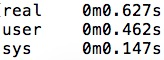
\includegraphics
	[width=0.3\textwidth]{time.jpg} 
	\caption{Output of time}.
\end{figure}
\begin{description}
	\item[$\cdot$] Real: This is the wall time mentioned above.
	\item[$\cdot$] User: User time is how much CPU time is spent in user mode.
	\item[$\cdot$] Sys: System time is how much CPU time is spent in kernel mode.
\end{description}
The difference between user- and kernel mode is the following:\\
In most memory protected system there are some locked operations for security reasons. E.g. allocation of memory or accessing hardware requires kernel mode and cannot be done in user mode. Processes like malloc and reading / writing to files will somewhere in the process sent a request to the kernel to do certain things and this is counted as system time. This does not necessarily mean that all time is spent in kernel mode when reading a file, since the only time that is spent in kernel mode is accessing the requested data in memory the rest of the operation is counted towards user time.\\ 
\\
So to get much times is spent on the CPU, User time + system is a good estimation. To get an even better indication of the real CPU time, multiple test are done and the average is calculated. The average running time is considered since there can be fluctuations in run times for every test. \\
\\
Another way to measure time spent on the CPU is to use the built in libraries for example System.currentTimeMillis() in Java. This is especially useful for profiling and figuring out which part of a program is time consuming.
Benchmarking will be done by comparing CPU time of the same problem in different languages. The problems will be scaled to have smaller and larger inputs. However, in some situations a large input can cause memory problems, which will be addressed in the specific problem. The memory problems is unfortunately making an upper bound for how large data is possible to pass for certain problems. \\
\\
The algorithm used for a given problem is the same used in all compared languages. Extended tests will be included for which the algorithm is optimized for a given language.

\section{Projecteuler 11}

\textit{In the 20x20 grid below, four numbers along a diagonal line have been marked in red. The product of these numbers is 26 x 63 x 78 x 14 = 1788696. What is the greatest product of four adjacent numbers in the same direction (up, down, left, right, or diagonally) in the 20x20 grid?}
\begin{figure}[H]
	\begin{center}
	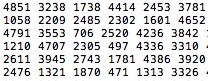
\includegraphics[scale=0.80]{11.jpg}
	\label{11}
	\end{center}
\end{figure}
The program runs from command-line/terminal with command line arguments in order to be able to test on different inputs and amount of adjacent numbers multiplied. To run the Julia version from the terminal: \\
\textbf{Julia euler11.jl 100 4}. \\
This would make the program run with a matrix of size 100 and calculating product of 4 adjacent numbers. A matrix generator was created, which can be found in appendix, to produce the matrix data. The matrix generator requires one argument, which is the size of the matrix. So if 500 is passed to the matrix generator, a file named 500mat.txt will be created containing 500x500 digits ranging from 100-9999.\\
\\
The algorithm first reads through the input file and creates a matrix. To calculate products in all directions needed in the problem, the algorithm goes through the matrix a total of 3 times. A nested for loop is needed to go though a matrix, lines 1-2 at figure \ref{111}. The outer loop iterates through the rows, and the inner loop iterates through the columns. Figure \ref{111} calculates the horizontal and vertical directions, firgure \ref{112} diagonally from left to right(downwards) and figure \ref{113} going diagonally from right to left(downwards). The algorithm starts in the most upper left cell, and iterates through all cells in the matrix. Lets have the first cell as (1,1), first number is row(\textbf{i}) and second number is column(\textbf{j}). Looking at figure \ref{111}, \textbf{matLength} is the size of the matrix, size = 100 would mean a matrix of size $100 \cdot 100$. \textbf{numProd} is the number of adjacent numbers multiplied together. For matrix with size 100, and multiplying four adjacent numbers, the algorithm would do the following in figure \ref{111}: 
\begin{list}{}{}
	\item Starting at cell (1,1) to the end which is cell (100, 100 - 4).
	\item Line 5-7: Loops over the adjacent cells and multiplies the numbers.
	\item Line 8-10: Sets current product to max product, if current is larger than previously max product.
\end{list}
\begin{figure}[H]
	\begin{center}
		\lstinputlisting[linerange={22-38}]{euler11.jl}
		\caption{Horizontal and vertical}
		\label{111}
	\end{center}
\end{figure}
Figure \ref{112} shows the loop that iterates over the matrix and calculating the product of the diagonal going downwards from left to right. Figure \ref{113} shows the diagonal product going upwards from left to right. The loop starts in the first row, and starting column is the last, not the first like the previously loops.
\begin{figure}[H]
	\begin{center}
		\lstinputlisting[linerange={43-51}]{euler11.jl}
		\caption{Diagonal downwards left to right}
		\label{112}
	\end{center}
\end{figure}
\begin{figure}[H]
	\begin{center}
		\lstinputlisting[linerange={56-64}]{euler11.jl}
		\caption{Diagonal upwards left to right}
		\label{113}
	\end{center}
\end{figure}

\section{Projecteuler 116}
Description: A row of five black square tiles is to have a number of its tiles replaced with coloured oblong tiles from red(length two), green(length three), or blue(length four). If red tiles are chosen there are exactly seven ways. If green tiles are chosen there are three ways. And if blue tiles are chosen there are two ways. Figure \ref{116} is a visualization of how the tiles can be lain. Assuming that colours cannot be mixed there are $7+3+2=12$ ways of replacing the black tiles in a row measuring five units in length. How many different ways can the black tiles in a row measuring fifty units in length be replaced if colours cannot be mixed and at least one coloured tile must be used?

\begin{figure}[H]
	\centering
	\begin{subfigure}[b]{0.6\textwidth}
		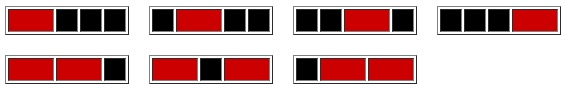
\includegraphics
		[width=\textwidth]{1161.jpg}
		\caption{Red tiles}.
	\end{subfigure}
	\begin{subfigure}[b]{0.6\textwidth}
		\centering
		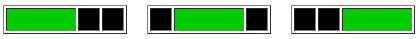
\includegraphics
		[width=\textwidth]{1162.jpg} 
		\caption{Green tiles}.
	\end{subfigure}	
	\begin{subfigure}[b]{0.6\textwidth}
		\centering
		
\includegraphics
		[width=\textwidth]{1163.jpg} 
		\caption{Blue tiles}.
	\end{subfigure}
	\caption{Projecteuler: 116}
	\label{116}
\end{figure}


\section{Quicksort}
Quicksort applies the divide-and-conquer paradigm to sort numbers. Divide-and-conquer has three steps. \textbf{Divide} the problem into a number of subproblems that are smaller instances of the same problem. \textbf{Conquer} the subproblems by solving them recursively. If the subproblems sizes are small enough, however, just solve the subproblems in a straightforward manner. \textbf{Combine} the solutions to the subproblems into the solution for the original problem \cite[chapter 4, page 65]{cormen}. Description of quicksort: \cite[chapter 7, page 170-171]{cormen}
\begin{list}{}{}
	\item \textbf{Divide}: Partition (rearrange) the array A[p..r] into two (possible empty) subarrays A[p..q-1] and A[q+1..r] such that each element of A[p--q1] is less than or equal to A[q], which is, in turn, less than or equal to each element of A[q+1..r]. Compute the index q as part of this partitioning procedure.
	\item \textbf{Conquer}: Sort the two subarrays A[p..q-1] and A[q+1..r] by recursive calls to quicksort.
	\item \textbf{Combine}: Because the subarrays are already sorted, no work is needed to combine them: the entire array A[p..r] is now sorted.
\end{list}
Figure \ref{qs} shows a visualization of quicksort.
\begin{figure}
	\begin{center}	
		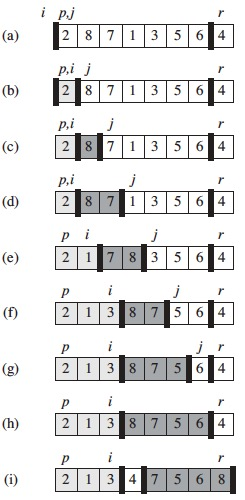
\includegraphics[scale=0.5]{qs.jpg}
		\caption{Quicksort}
		\label{qs}
	\end{center}
\end{figure}

\section{Statistics}

\section{Learning / Personal experience}
Some of the design choices, in Julia, can be really frustrating for someone who is adapting to Julia. The indexes starts at 1 - this could be debatable because of the statement that Julia is used in a lot of scientific computations and many programming languages made for scientific computations starts at index 1. But as a programmer who is used to indexes starting at 0, this can cause a lot of unnecessary bugs. The developers of Julia also made a weird design choice with the for-loop syntax. A incrementing for loop looks like:
\begin{lstlisting}[language=python]
Julia:
for i = 1 : n
	Some code ...
end

General languages:
for i = 1; i < n; i++
	Some code ...
\end{lstlisting}
This is straightforward like many other languages, but take a look at the decrementing for-loop:
\begin{lstlisting}[language=python]
Julia:
for i = n : -1 : 0
	Some code ...
end

General languages:
for i = n; i > 0; i--
	Some code
\end{lstlisting}
In Julia the exit condition and incrementation / decrementation are swapped and there is no consistency. The decrementing for-loops both start at n, and stops at 0. This kind of syntax can again cause bugs, and is not that easy to get eyes on.\\
\\
The documentation of Julia is far from being great, which is a huge bump on the road to learn Julia. It feels far from complete. The documentation do not explain much but instead gives some examples. Essential information are often lacking, e.g. what types is needed to parse for a given function. It might point out that these arguments are needed, but lacking to describe those arguments. An example from the documentation is the function \textbf{rand()} which is used to generate random numbers:

\begin{lstlisting}
rand( [ rng ] [ ,S ] [ , dims... ] )

	Pick a random element or array of random elements from the set of values specified by S; S can be:
	- an indexable collection (for example 1:n or ['x','y','z']), or  
	- a type: the set of values to pick from is then equivalent to typemin(S):typemax(S) for integers (this is not applicable to BigInt), and to [0,1) for floating point numbers;  
	S defaults to Float64.
\end{lstlisting} 
The argument \textbf{S} is explained, but does not mention anything about \textbf{rng} or \textbf{dims}.\\
Antoher example is how to access data within an array at a specific index. This should be one of the first things in the Array section, but is first described after about two pages of text. A person with experience in programming might know that to access an element in an array with an index is this simple line of code:
\begin{lstlisting}
a[index]
\end{lstlisting} 
But this isn’t so obvious for new programmers. It is clear that something has to be done with the documentation.\\
\\ 
Another downside to Julia is its consistency. The developers has tried to remove some of the burden from the programmer with dynamic typing, package manager system etc., but with memory allocation and garbage collection it does not make much sense. The garbage collector does not free memory from unreachable object. Sizes of variables cannot be changed after declaration, and is not automatically increased if needed. If the programmer assign for example 8 bit memory to a variable and later change the value of that variable, then julia automatically assigns 32 bit or more if needed to that variable even if the 8 bits were enough. 

\section{Conclusion}
It can be difficult to make any conclusions by the benchmarking but it may give an idea of how Julia performs, compared to Java, Python and C++. One thing to keep in mind is that as of writing this report, Julia is in version 0.4.5 - it has yet to reach version 1.0.0 while the other languages are much older than Julia. This could mean that Julia might get even faster in the future.   

\newpage

\section{Appendix (source code)}

%\textbf{Sierpinski triangle program}
%\lstinputlisting[language=python]{sierpinski.py}
%\textbf{Binary tree program}
%\lstinputlisting[language=python]{binary.py}

\begin{thebibliography}{9}
	
	\bibitem{cormen}
	Thomas H. Cormen, Charles E. Leiserson, Ronald Rivest, Clifford Stein
	\emph{Introduction to Algorithms},
	Cambridge, Massachusetts,
	third edition,
	2009.
	
\end{thebibliography}

\end{document}

